\subsection{Comparison of results between Newton's method and MM2}

\begin{center}
   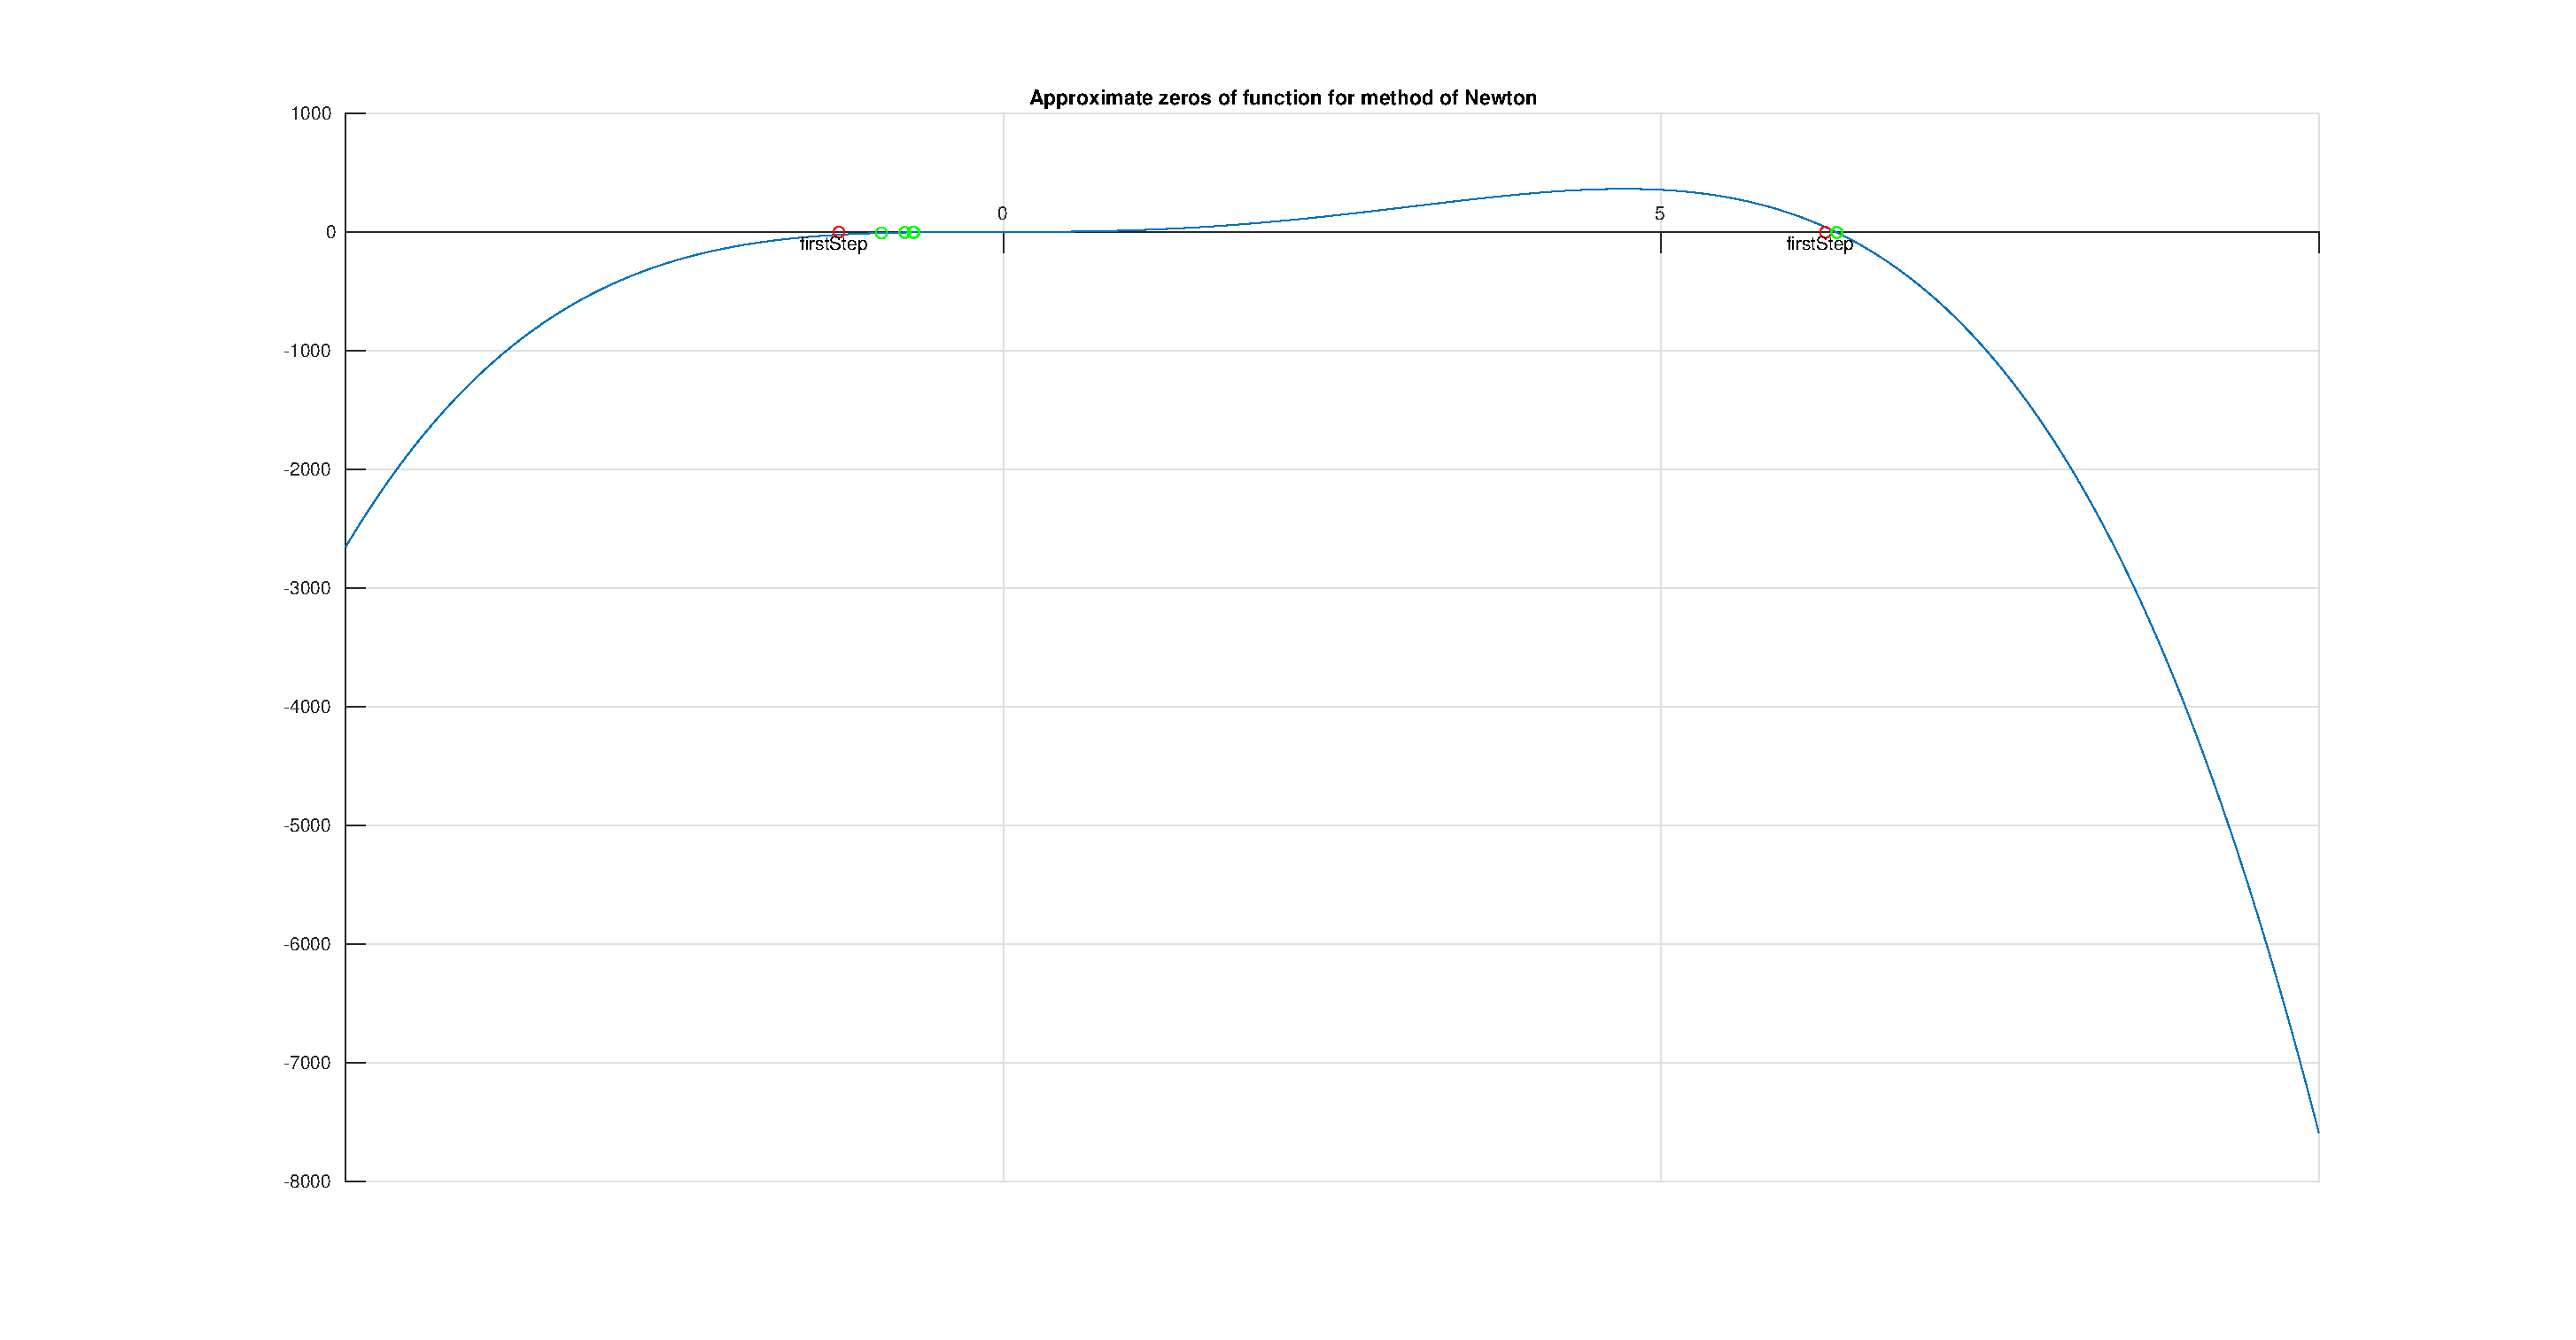
\includegraphics[scale=0.25]{task2newtonoverall.eps}
\end{center}

\begin{center}
   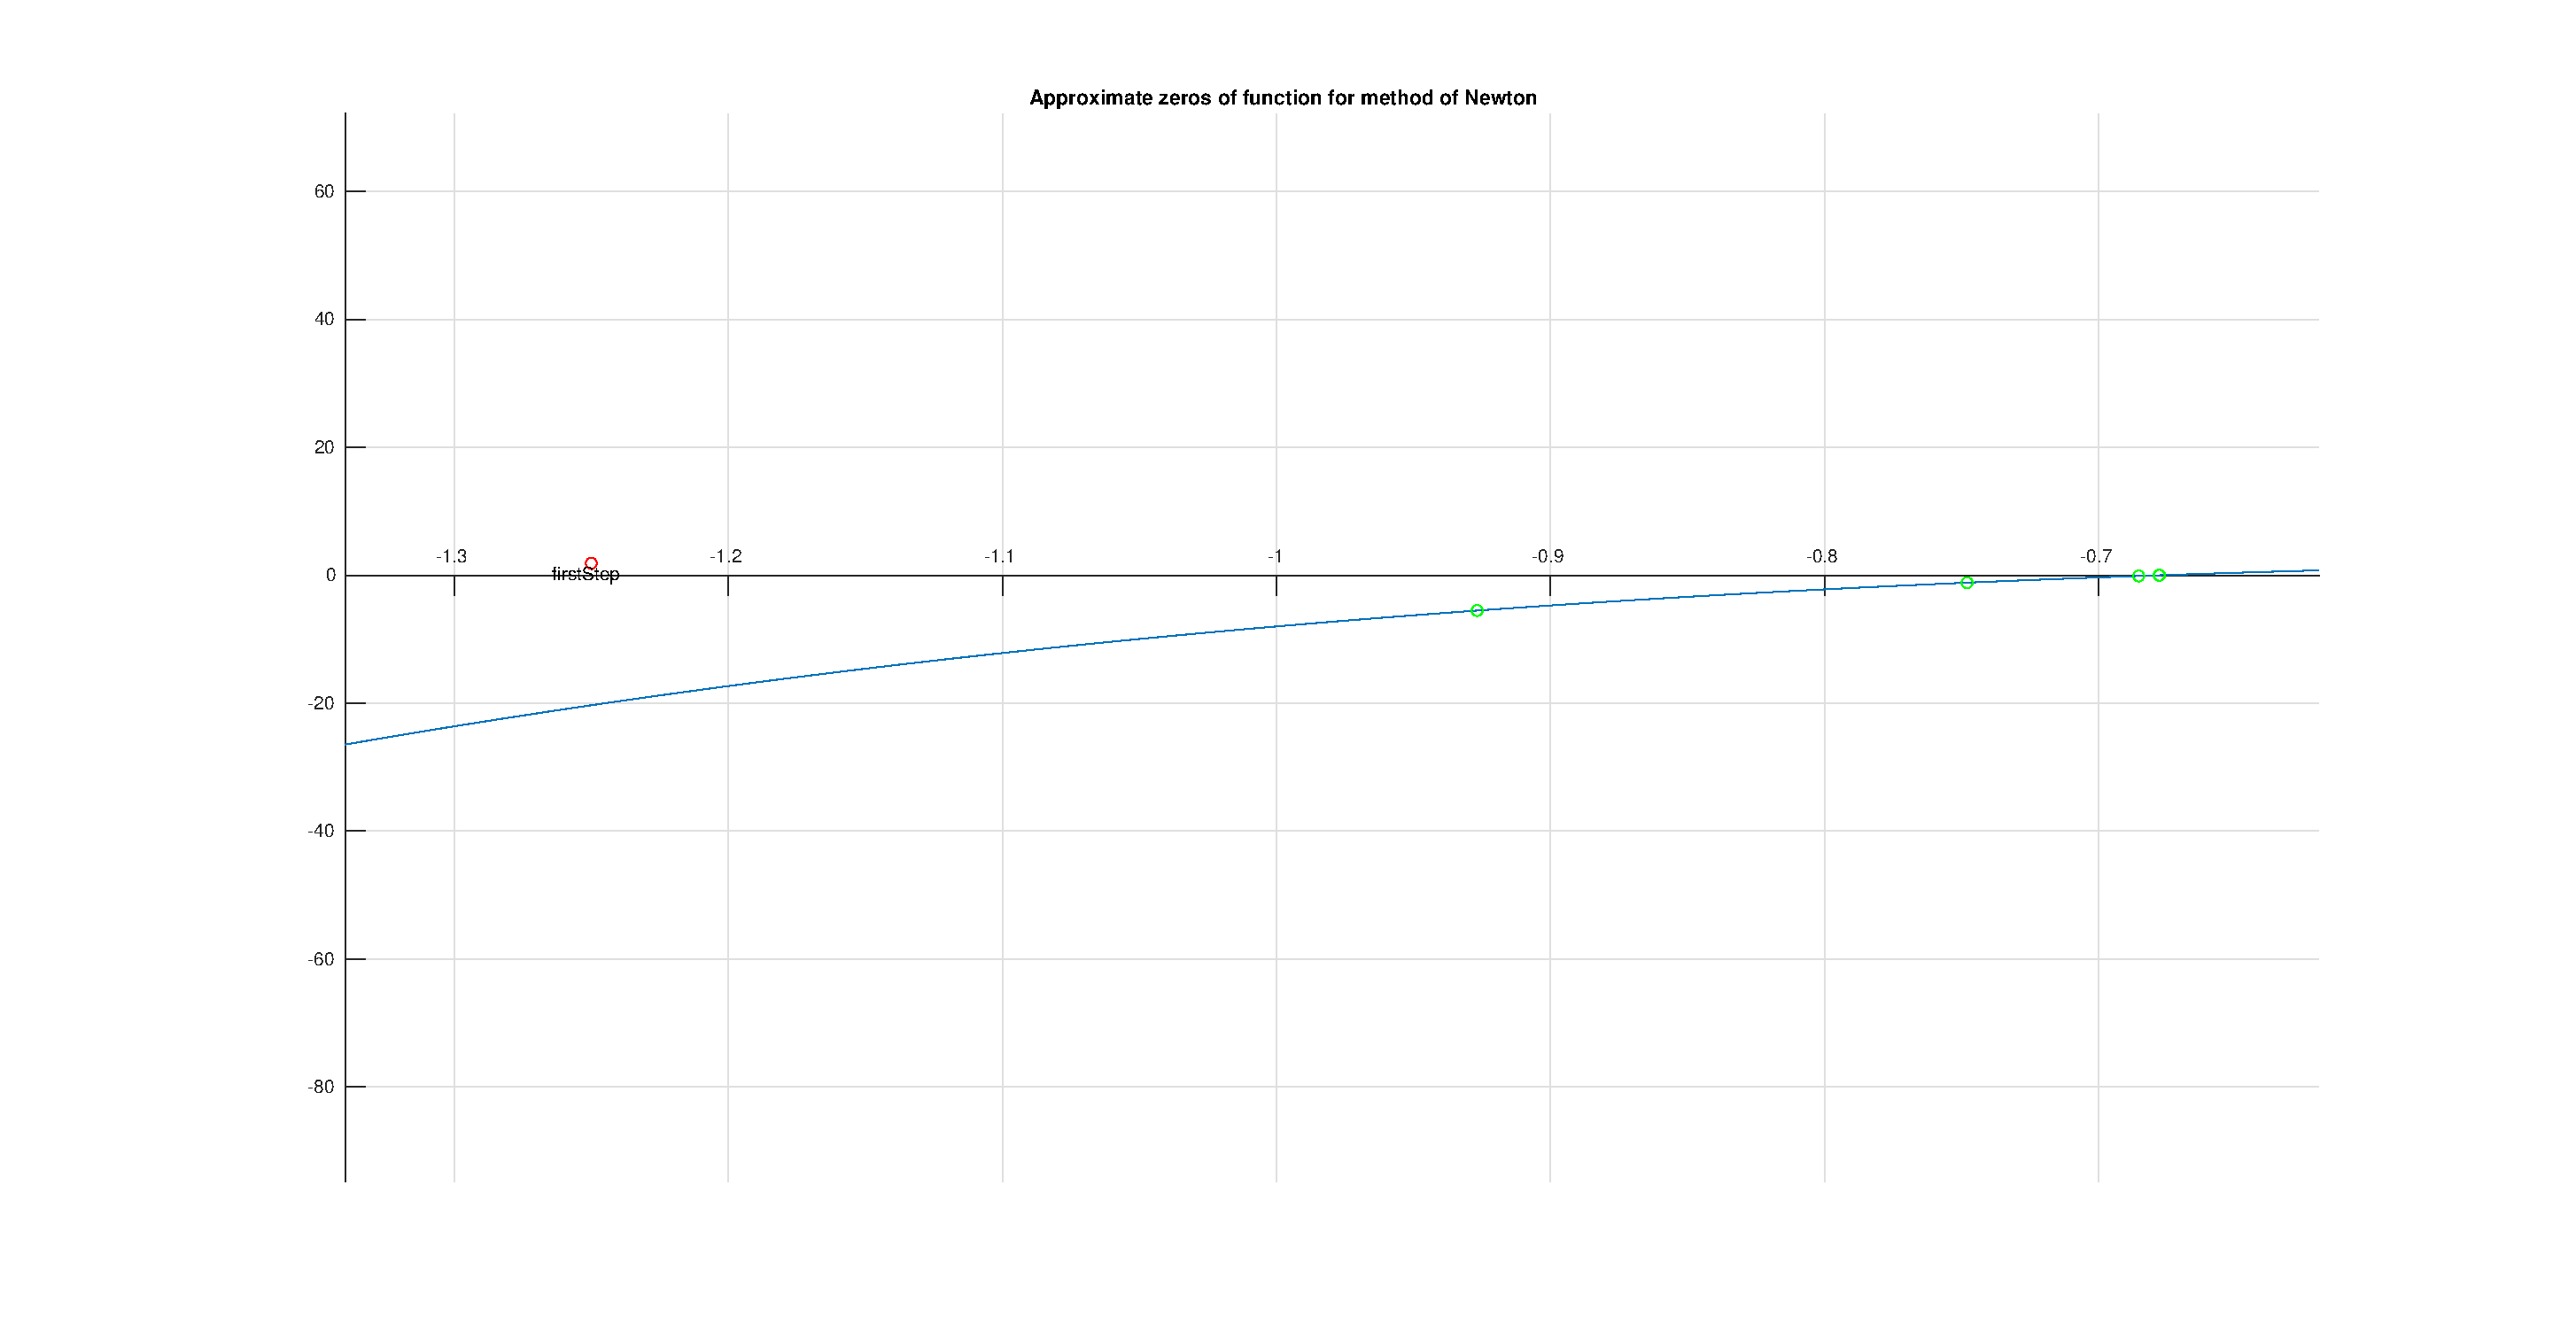
\includegraphics[scale=0.25]{task2newtonleft.eps}
\end{center}

\begin{center}
   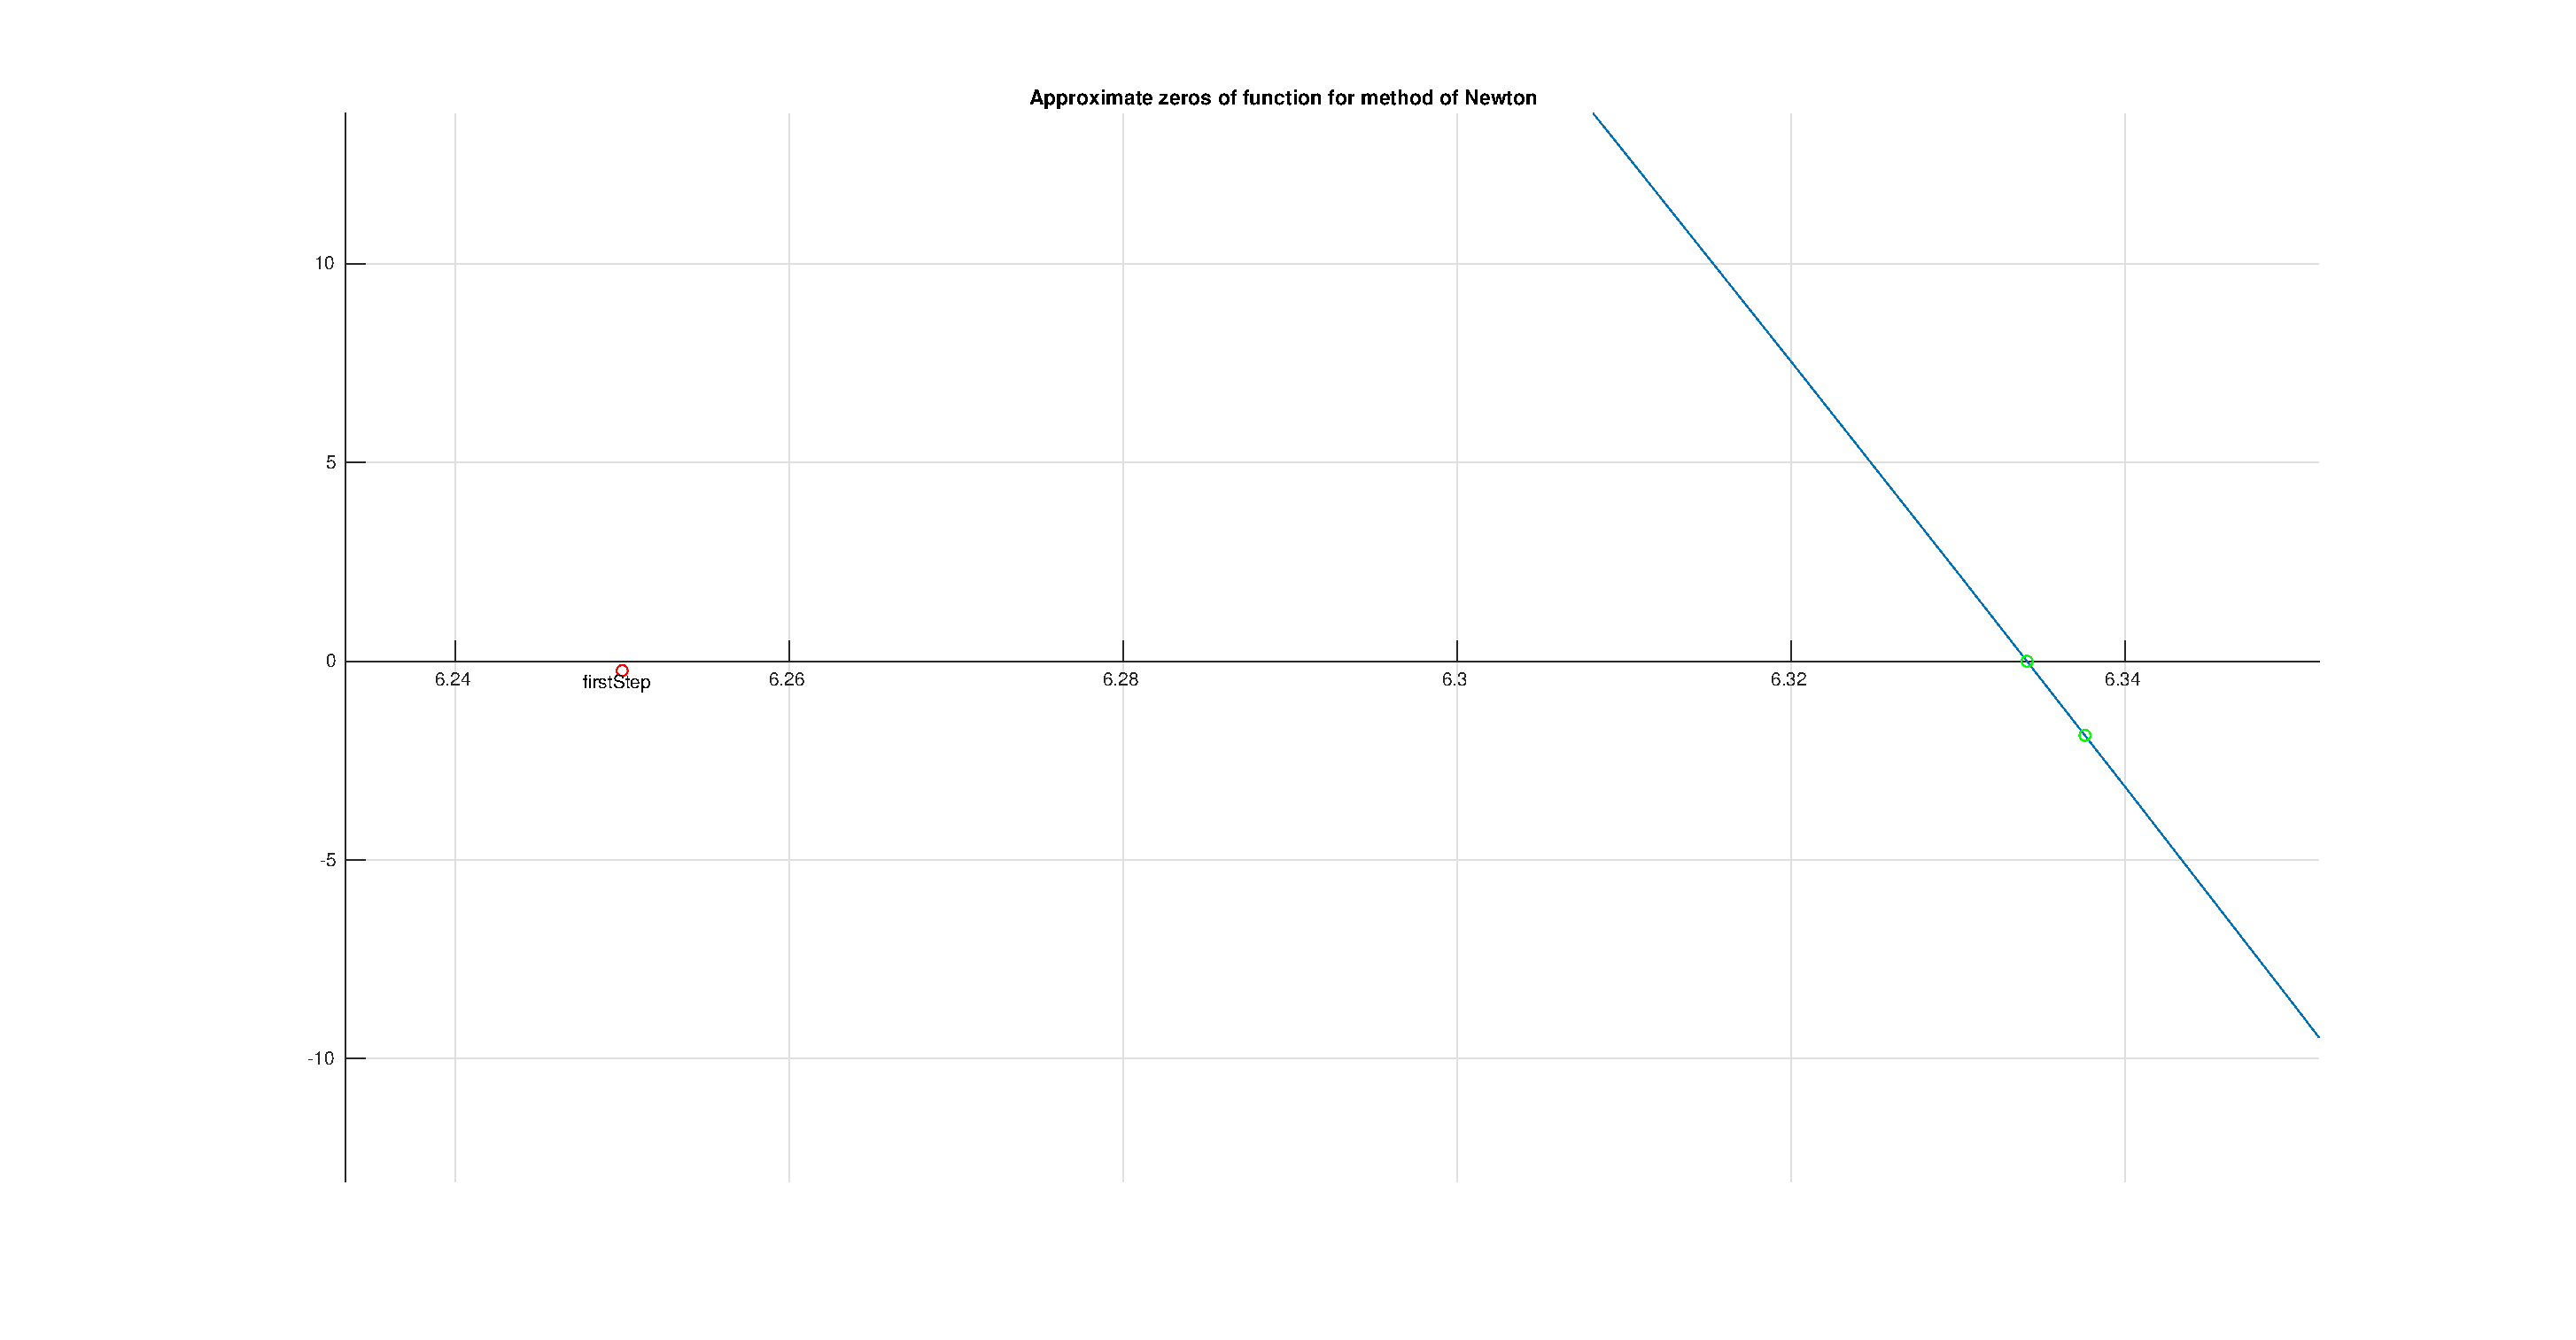
\includegraphics[scale=0.25]{task2newtonright.eps}
\end{center}


\begin{center}
  \begin{tabular}{| c  c c |}
\hline
Iteration & root         & f(root) \\
\hline
 1  &       -1.25   &       1.8879 \\
 \hline
 2  &    -0.92681  &         -5.52 \\
 \hline
 3  &   -0.74804   &       -1.159 \\
 \hline
 4  &   -0.68543   &     -0.11186 \\
 \hline
 5  &   -0.67797   &   -0.0014548 \\
 \hline
 6  &    -0.67787  &    -2.568e-07 \\
 \hline
 7  &   -0.67787   & -7.9936e-15 \\
 \hline
\end{tabular}
\end{center}

\begin{center}
  \begin{tabular}{| c  c c |}
\hline
Iteration & root         & f(root) \\
\hline
 1   &     6.25   &     -0.23707 \\
 \hline
 2   &   6.3376   &      -1.8647 \\
 \hline
 3   &  6.3341    &  -0.0029912 \\
 \hline
 4   &   6.3341   & -7.7134e-09 \\
 \hline
 5   &   6.3341   &  -7.1942e-14 \\
 \hline
\end{tabular}
\end{center}

As we can see Newton method calculated real roots in around the same number of iterations as method MM1, it was slightly slower than MM2. Newton method had pretty good accuracy, comparable to MM1 accuracy.


\chapter{Find real and complex roots of the polynomial using Laguerre's method}

